\documentclass[
  bibliography=totoc,     % Literatur im Inhaltsverzeichnis
  captions=tableheading,  % Tabellenüberschriften
  titlepage=firstiscover, % Titelseite ist Deckblatt
]{scrartcl}

% Paket float verbessern
\usepackage{scrhack}

\setlength{\parindent}{0em}

% Warnung, falls nochmal kompiliert werden muss
\usepackage[aux]{rerunfilecheck}

% unverzichtbare Mathe-Befehle
\usepackage{amsmath}
% viele Mathe-Symbole
\usepackage{amssymb}
% Erweiterungen für amsmath
\usepackage{mathtools}

% Fonteinstellungen
\usepackage{fontspec}
% Latin Modern Fonts werden automatisch geladen
% Alternativ zum Beispiel:
%\setromanfont{Libertinus Serif}
%\setsansfont{Libertinus Sans}
%\setmonofont{Libertinus Mono}

% Wenn man andere Schriftarten gesetzt hat,
% sollte man das Seiten-Layout neu berechnen lassen
\recalctypearea{}

% deutsche Spracheinstellungen
\usepackage{polyglossia}
\setmainlanguage{german}


\usepackage[
  math-style=ISO,    % ┐
  bold-style=ISO,    % │
  sans-style=italic, % │ ISO-Standard folgen
  nabla=upright,     % │
  partial=upright,   % ┘
  warnings-off={           % ┐
    mathtools-colon,       % │ unnötige Warnungen ausschalten
    mathtools-overbracket, % │
  },                       % ┘
]{unicode-math}

% traditionelle Fonts für Mathematik
\setmathfont{Latin Modern Math}
% Alternativ zum Beispiel:
%\setmathfont{Libertinus Math}

\setmathfont{XITS Math}[range={scr, bfscr}]
\setmathfont{XITS Math}[range={cal, bfcal}, StylisticSet=1]

% Zahlen und Einheiten
\usepackage[
  locale=DE,                   % deutsche Einstellungen
  separate-uncertainty=true,   % immer Fehler mit \pm
  per-mode=symbol-or-fraction, % / in inline math, fraction in display math
]{siunitx}

% chemische Formeln
\usepackage[
  version=4,
  math-greek=default, % ┐ mit unicode-math zusammenarbeiten
  text-greek=default, % ┘
]{mhchem}

% richtige Anführungszeichen
\usepackage[autostyle]{csquotes}

% schöne Brüche im Text
\usepackage{xfrac}

% Standardplatzierung für Floats einstellen
\usepackage{float}
\floatplacement{figure}{htbp}
\floatplacement{table}{htbp}

% Floats innerhalb einer Section halten
\usepackage[
  section, % Floats innerhalb der Section halten
  below,   % unterhalb der Section aber auf der selben Seite ist ok
]{placeins}

% Seite drehen für breite Tabellen: landscape Umgebung
\usepackage{pdflscape}

% Captions schöner machen.
\usepackage[
  labelfont=bf,        % Tabelle x: Abbildung y: ist jetzt fett
  font=small,          % Schrift etwas kleiner als Dokument
  width=0.9\textwidth, % maximale Breite einer Caption schmaler
]{caption}
% subfigure, subtable, subref
\usepackage{subcaption}

% Grafiken können eingebunden werden
\usepackage{graphicx}
% größere Variation von Dateinamen möglich
\usepackage{grffile}

% schöne Tabellen
\usepackage{booktabs}

% Verbesserungen am Schriftbild
\usepackage{microtype}

% Literaturverzeichnis
\usepackage[
  backend=biber,
]{biblatex}
% Quellendatenbank
\addbibresource{lit.bib}
\addbibresource{programme.bib}

% Hyperlinks im Dokument
\usepackage[
  unicode,        % Unicode in PDF-Attributen erlauben
  pdfusetitle,    % Titel, Autoren und Datum als PDF-Attribute
  pdfcreator={},  % ┐ PDF-Attribute säubern
  pdfproducer={}, % ┘
]{hyperref}
% erweiterte Bookmarks im PDF
\usepackage{bookmark}

% Trennung von Wörtern mit Strichen
\usepackage[shortcuts]{extdash}

\author{%
  Sara Krieg\\%
  \href{mailto:sara.krieg@udo.edu}{sara.krieg@udo.edu}%
  \texorpdfstring{\and}{,}%
  Marek Karzel\\%
  \href{mailto:marek.karzel@udo.edu}{marek.karzel@udo.edu}%
}
\publishers{TU Dortmund – Fakultät Physik}


\subject{Nr. 401}
\title{Das Michelson-Interferometer}
\date{%
  Durchführung: 18.06.2019
  \hspace{3em}
  Abgabe: 25.06.2019
}

\begin{document}

\maketitle
\thispagestyle{empty}
\tableofcontents
\newpage

\section{Theorie}
\label{sec:Theorie}

Bei diesem Versuch soll die Temperaturabhängigkeit der dynamischen 
Viskosität von destilliertem Wasser mit Hilfe der Kugelfall Methode nach 
Höppler ermittelt werden. Dazu wird die Apperaturkonstante des 
verwendeten Viskosimeters ermittelt. Es muss desweiteren mit Hilfe der 
Reynoldzahl überprüft werden, ob laminare Strömungsverhältnisse gegeben 
sind. \\
\\Zunächst werden die Kräfte betrachtet, die auf einem Körper wirken, der
sich durch eine Flüssigkeit bewegt: 

\begin{equation}
F_{ges} = F_g - F_a - F_r
\end{equation}

Dabei bezeichnet $F_g$ die Gravitationskraft, $F_a$ die Auftriebskraft und 
$F_r$ die Reibungskraft, welche hier zunächst ohne Beweis als Stokesche 
Reibung angenommen wird. Somit ergibt sich: 

\begin{equation}
F_{ges} = \rho _K\cdot V_K\cdot g - (\rho _K - \rho _F)\cdot V_K - 6\pi\cdot \eta \cdot v\cdot r
\end{equation}

Dabei ist $\rho _K$ die Dichte der Kugel, $V_K$ das Volumen der Kugel, 
$\rho _F$ die Dichte der verwendeten Flüssigkeit, $\eta$ die Viskosität, 
$v$ die Geschwindigkeit mit der die Kugel fällt und $r$ ihr Radius. 
Die Geschwindigkeit $v$ wird konstant, sobald sich ein Kräftegleichgewicht 
zwischen den wirkenden Kräften einstellt. \\
\\Der Begriff Viskosität $\eta$ lässt sich als "Zähflüssigkeit" interpretieren.
Diese Größe ist materialabhängig, was intuitiv klar ist, wenn man betrachtet, 
dass sich zum Beispiel Honig sehr viel zähflüssiger bewegt als Wasser, was bedeutet, 
dass die Viskosität von Honig weitaus höher ist. 
Demnach werden Bewegungen von Flüssigkeiten durch die dynamische Viskosität dieser 
charakterisiert. 
Bestimmen lässt sich $\eta$ zum Beispiel mit dem Kugelfallviskosimeter nach 
Höppler, welches hier verwendet wird. Dabei gilt die folgende empirische Gleichung: 

\begin{equation}
\eta = K\cdot (\rho _K - \rho _F)\cdot t
\label{eqn:Viskosität}
\end{equation}

Mit der Falldauer $t$, sowie der Apperaturkonstanten $K$.
Die dynamische Viskosität wird als dynamisch bezeichnet, weil sie stark 
temperaturabhängig ist. Häufig gilt die Andradesche Gleichung:

\begin{equation}
\eta (T) = A\cdot exp(\frac{B}{T})
\end{equation}

Dabei sind A und B Konstanten. 

Diese Zusammenhänge gelten allerdings nur für sogenannte "Newtonsche Fluide",
in denen der Geschwindigkeitsverlauf linear ist. Vorraussetzung für solche 
Fluide sind laminare Strömungsverhältnisse, bei denen die Flüssigkeitsschichten
wirbelfrei aneinander abgleiten. Erst wenn solche Strömungsverhältnisse gegeben 
sind, kann die Reibungskraft als Stokesche Reibung angenommen werden. 
Ob eine Strömung laminar oder turbulent ist, kann anhand der Reynolds-Zahl 
abgeschätzt werden. 

\begin{equation}
Re = \frac{\rho _F\cdot v_m\cdot 2r}{\eta}
\label{eqn:Reynolds}
\end{equation}

Dabei bezeichnet $\rho _F$ die Dichte und $\eta$ die Viskosität der Flüssigkeit. 
$v_m$ ist die mittlere Geschwindigkeit der Kugel und $r$ ihr Radius.
Erhält man für $Re$ einen Wert, der unter 2000 liegt, so kann man davon ausgehen, 
dass die Strömung laminar ist. 

\cite{sample}

\section{Durchführung}
\label{sec:Durchführung}

Um die spezifischen Wärmekapazitäten $C_V$ der beiden Festkörperproben (Aluminium und Kupfer)
genau bestimmen zu können,
muss in einer vorbereitenden Messung erst die Wärmekapazität des Kalorimeters $c_gm_g$ bestimmt werden,
um die an die Wände des Kalorimeters abgegebene Wärmemenge in die Ermittlung der Wärmekapazitäten der
Festkörperproben einbeziehen zu können.

Dazu müssen, wie aus Gleichung \ref{eqn:KapKalori} ersichtlich,
erst die Massen $m_x$, $m_y$ der beiden Wasserproben mittels einer feinen Waage bestimmt werden.
Dabei ist darauf zu achten, dass die Masse der Bechergläser nicht mit eingerechnet wird. 
Anschließend wird eine der Wasserproben auf einer Heizplatte erhitzt und schließlich werden die
Temperaturen $T_x$, $T_y$ der Proben mithilfe eines Thermoelements gemessen.
Zuletzt werden beide Wasserproben in das Kalorimeter gegossen und die sich einstellende Mischtemperatur 
$T_m$ gemessen, sobald sich das thermische Gleichgewicht eingestellt hat.
Zur Beschleunigung des Vorgangs wird ein Magnetrührer verwendet.

Die verbleibende Größe, die Wärmekapazität des Wassers $c_w$, muss nicht bestimmt werden, sondern ist mit
$\SI{4.18}{\joule\per\gram\cdot\kelvin}$ bei ca. $\SI{40}{\celsius}$ Wassertemperatur angegeben.


Nun wird eine, ähnlich zu der zuvor beschriebenen, Messung zur Bestimmung der spezifischen Wärmekapazitäten
$C_V$ von Aluminium und Kupfer durchgeführt. Hierzu muss zunächst jeweils die Masse $m_k$ des Probekörpers
und die Masse $m_w$ des Wassers mit einer feinen Waage bestimmt werden.
Anschließend wird die Probe in einem Wasserbad auf einer Heizplatte auf ca. $\SI{100}{\celsius}$ erhitzt. 
Daraufhin wird die Probe dem Wasserbad entnommen und die Temperaturen $T_k$ und $T_w$ des Probekörpers
und des Wassers gemessen.
Schließlich werden das Wasser und die Probe in das Kalorimeter gegeben und erneut wird die sich einstellende
Mischtemperatur $T_m$ gemessen.

Die zweite Messung wird für Aluminium einmal, für Kupfer dreimal durchgeführt. Aus den gemessenen
Größen kann nun nach Gleichung \ref{eqn:KapProbe} die jeweilige spezifische Wärmekapazität des Stoffes
berechnet werden.










\section{Auswertung}
\label{sec:Auswertung}

\subsection{Untersuchung der Filterkurve}

Zunächst wird die Durchlassfrequenz $\nu$ des Selektivverstärkers bestimmt. Die 
gemessenen Wertepaare von Frequenz $\nu$ und Spannung $U_\text{A}$ sind in 
Tabelle \ref{tab:Messdaten1} aufgeführt. 

\begin{table}
\centering
\caption{Messwerte der Filterkurve des Selektivverstärkers.}
\label{tab:Messdaten1}
\sisetup{table-format=2.1}
\begin{tabular}{c c c c}
\toprule
$\nu \,/\, \si{\kilo\hertz}$ & $U_\text{A} \,/\, \si{\milli\volt}$ & $\nu \,/\, \si{\kilo\hertz}$ & $U_\text{A} \,/\, \si{\milli\volt}$\\
\midrule
20,0 &  0,865 & 34,6 & 35,00\\
21,0 &  0,900 & 34,7 & 43,00\\
22,0 &  0,990 & 34,8 & 55,00\\
23,0 &  1,095 & 34,9 & 72,50\\
24,0 &  1,230 & 35,0 & 93,00\\
25,0 &  1,380 & 35,1 & 96,00\\
26,0 &  1,560 & 35,2 & 78,00\\
27,0 &  1,800 & 35,3 & 59,00\\
28,0 &  2,100 & 35,4 & 46,00\\
29,0 &  2,520 & 35,5 & 37,00\\
30,0 &  3,200 & 35,6 & 31,00\\
31,0 &  4,000 & 35,7 & 26,00\\
32,0 &  5,450 & 35,8 & 23,00\\
33,0 &  8,350 & 35,9 & 20,00\\
34,0 & 16,000 & 36,0 & 18,00\\
34,1 & 17,000 & 36,1 & 16,00\\
34,2 & 19,500 & 37,0 &  9,00\\
34,3 & 22,000 & 38,0 &  6,15\\
34,4 & 25,000 & 39,0 &  4,60\\
34,5 & 29,000 & 10,0 &  3,70\\
\bottomrule
\end{tabular}
\end{table}

Die gemessene Frequenz $\nu$ wird gegen die Spannung $U_\text{A}$ aufgetragen. Das 
Ergebnis ist in Abbildung \ref{fig:plot1} zu finden. 

\begin{figure}
  \centering
  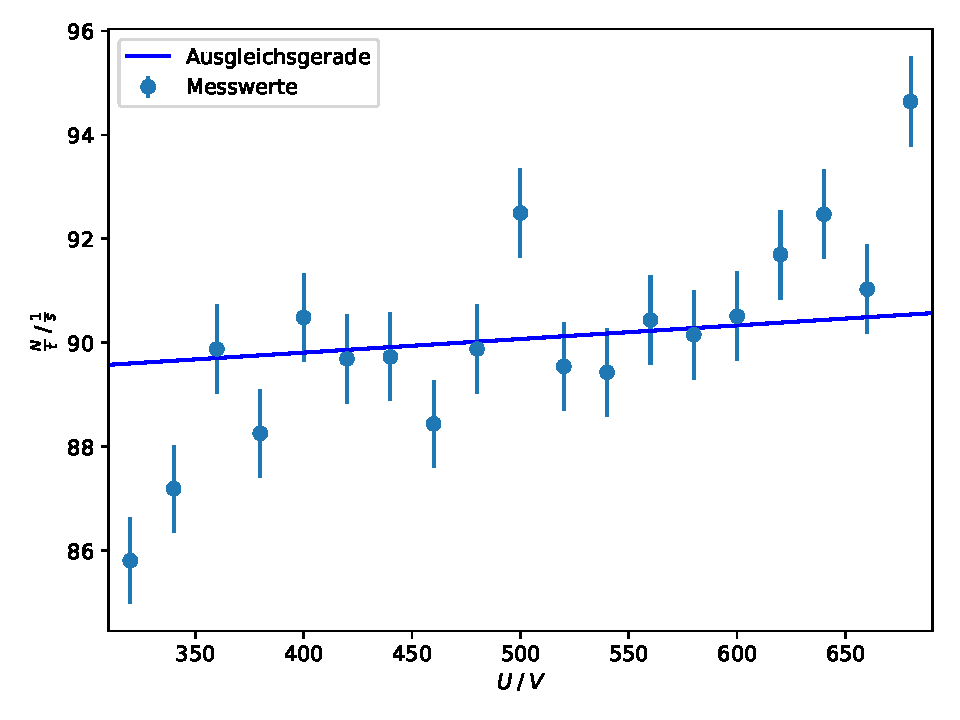
\includegraphics{content/plot1.pdf}
  \caption{Filterkurve des Selektivverstärkers.}
  \label{fig:plot1}
\end{figure}

Mittels Python 3.6.5. und dem Paket Matplotlib wird eine Lorentzkurve für eine Ausgleichskurve 
gefittet. Dabei wird die Gleichung 

\begin{equation*}
f(x) = \frac{a}{(x²-x_0^2)²+\gamma²x_0²}
\end{equation*}

für die berechnete Lorentzkurve und die Werte von $\SI{34.1}{\kilo\hertz}$ bis $\SI{36.0}{\kilo\hertz}$verwendet. 

Die Durchlassfrequenz lässt sich nun direkt ablesen und ergibt sich zu:

\begin{equation}
x_0 = \nu _\text{A} = \SI{35.065}{\kilo\hertz}.
\end{equation}

Desweiteren wird bei einem Wert von $\frac{1}{\sqrt{2}}$ des Maximalwerts
eine Gerade angelegt. Die Parameter ergeben sich schließlich zu: 

\begin{align*}
a &= \SI{6.6+-0.4e4}{\volt\per\second²},\\
\gamma &= \SI{0.772+-0.03}{}.
\end{align*}

Außerdem werden $\nu_\text{A}$, $\nu_1$ und $\nu_2$ mittels Python zu

\begin{align*}
\nu_1 &= \SI{34.816+-0.01}{\kilo\hertz},\\
\nu_\text{A} &= \SI{35.065+-0.01}{\kilo\hertz},\\
\nu_2 &= \SI{35.313+-0.01}{\kilo\hertz}
\end{align*}

berechnet. Die Güte $Q$ kann nun mit 

\begin{equation*}
Q = \frac{\nu_\text{A}}{\nu_2 - \nu_1}
\end{equation*}

zu 

\begin{equation*}
Q = \num{70.5+-2.8}
\end{equation*}

berechnet werden.
Der Fehler ergibt sich dabei durch eine Fehlerrechnung mittels 
Python.

\subsection{Theoretische Bestimmung der Suszeptibilitäten}

Nach Formel \eqref{eqn:theo} lassen sich die Theoriewerte Seltener 
Erde Verbindungen berechnen. Es werden $\symup{Dy_2O_3}$, $\symup{C_6O_{12}Pr_3}$, 
$\symup{Gd_2O_3}$ und $\symup{Nd_2O_3}$ untersucht. Es wird eine Temperatur von 
$T = \SI{294}{\kelvin}$ angenommen, was etwa Raumtemperatur entspricht.
Der Lande-Faktor $g_J$, sowie $S$, $L$ und $J$ sind in Tabelle \ref{tab:theo} 
aufgeführt.

\begin{table}
\centering
\caption{Theoretische Werte zur Berechnung der Suszeptibilitäten}
\label{tab:theo}
\sisetup{table-format=2.1}
\begin{tabular}{c c c c c}
\toprule
& $\symup{Nd_2O_3}$ & $\symup{Gd_2O_3}$ & $\symup{Dy_2O_3}$ & $\symup{C_6O_{12}Pr_3}$\\
\midrule
4f-Elektronen & 3    & 7   & 9    & 3\\
L             & 6    & 0   & 5    & 5\\
S             & 1,5  & 3,5 & 2,5  & 1\\
J             & 4,5  & 3,5 & 7,5  & 4\\
$g_J$         & 0,97 & 2,0 & 1,41 & 0,8\\
\bottomrule
\end{tabular}
\end{table}

Außerdem ergibt sich $N$ nach

\begin{equation*}
N = \frac{\rho}{M}\cdot N_\text{A}.
\end{equation*}

Dabei ist $N_\text{A} = \SI{6.02214129e23}{1\per\mol}$ [2] die 
Avogadrokonstante, $\rho$ die Dichte des jeweiligen Stoffes und $M$
die molare Masse. Diese Werte sind zusammen mit den berechneten Werten für $N$
in Tabelle \ref{tab:theo2} zu finden. Setzt man diese Werte alle in Gleichung  
\eqref{eqn:theo} ein, so ergeben sich die gesuchten Suszeptibilitäten, die sich ebenfalls in 
Tabelle \ref{tab:theo2} befinden. 

\begin{table}
\centering
\caption{Molare Masse $M$, die Zahl der magnetischen Momente
pro Volumeneinheit $N$ der Seltenen Erden Verbindungen und die berechneten 
Suszeptibilitäten $\chi$.}
\label{tab:theo2}
\sisetup{table-format=2.1}
\begin{tabular}{c c c c c}
\toprule
& $\symup{Nd_2O_3}$ & $\symup{Gd_2O_3}$ & $\symup{Dy_2O_3}$ & $\symup{C_6O_{12}Pr_3}$\\
\midrule
$M/\si{\gram\mol^-1}$            & 168     & 176    & 180    & 346\\
$N \cdot \num{e28}/\si{\meter³}$ & 2,60    & 2,53   & 2,61   & 1,09\\
$\chi$                           & 0,00536 & 0,0142 & 0,0294 & 0,00123\\
\bottomrule
\end{tabular}
\end{table}


\subsection{Experimentelle Bestimmung der Suszeptibilität}

Zunächst muss der Koeffizient Q durch den Querschnitt

\begin{equation}
Q_\text{real} = \frac{m}{\rho \cdot l}
\end{equation}

ersetzt werden. Dieser ergibt sich durch die Länge $l$, die Masse $m$ und 
die Dichte $\rho$ der Probe. Diesen Querschnitt müsste die Probe haben, wenn 
sie aus einem Einkristall bestünde.

\begin{table}
\centering
\caption{$Q_\text{real}$ der verwendeten Stoffe.}
\label{tab:Messdaten2}
\sisetup{table-format=2.1}
\begin{tabular}{c c}
\toprule
Stoff & $Q_\text{real} \,/\, \si{\centi\meter²}$\\
\midrule
$\symup{Gd_2O_3}$ & 0,119\\
$\symup{Dy_2O_3}$ & 0,121\\
$\symup{Nd_2O_3}$ & 0,078\\
$\symup{C_6O_\text{12}Pr_2}$ & 0,079\\
\bottomrule
\end{tabular}
\end{table}

Es wurde mit der Eingangsspannung $U_\text{E} = \SI{0.8}{\volt}$ gemessen. Der 
Spulenquerschnitt ist mit $F = \SI{86.6}{\milli\meter²}$ gegeben. Aus den Messwerten 
können nun die Suszeptibilitäten $\chi$ nach Formel \eqref{eqn:alternativ} berechnet werden, nach Bereinigung 
um die Verstärkung $V$. Diese finden sich in Tabelle \ref{tab:Messdaten3}, 
\ref{tab:Messdaten4}, \ref{tab:Messdaten5} und \ref{tab:Messdaten6}.
Dabei bezeichnen $U_\text{m}$ und $R_\text{m}$ die Spannung und Widerstände, 
während die Probe sich in der Spule befindet. $U_\text{0}$ und $R_\text{0}$
sind entsprechend die Werte ohne Probe in der Spule. 

\begin{table}
\centering
\caption{Messwerten und Suszeptibilitäten für $\symup{Dy_2O_3}$}
\label{tab:Messdaten3}
\sisetup{table-format=2.1}
\begin{tabular}{c c c c c}
\toprule
$U_\text{0} \,/\, \si{\milli\volt}$ & $R_\text{0} \,/\, \si{\ohm}$ & $U_\text{m} \,/\, \si{\milli\volt}$& $R_\text{m} \,/\, \si{\ohm}$ & $\chi _\text{exp}$ \\
\midrule
0,135 & 4,375 & 0,385 & 4,232 & 0,0020\\
0,090 & 4,425 & 0,150 & 4,255 & 0,0024\\
0,110 & 4,430 & 0,420 & 4,255 & 0,0025\\ 
\bottomrule
\end{tabular}
\end{table}

\begin{table}
\centering
\caption{Messwerten und Suszeptibilitäten für $\symup{Nd_2O_3}$}
\label{tab:Messdaten4}
\sisetup{table-format=2.1}
\begin{tabular}{c c c c c}
\toprule
$U_\text{0} \,/\, \si{\milli\volt}$ & $R_\text{0} \,/\, \si{\ohm}$ & $U_\text{m} \,/\, \si{\milli\volt}$& $R_\text{m} \,/\, \si{\ohm}$ & $\chi _\text{exp}$ \\
\midrule
0,10 & 4,255 & 0,08 & 4,455 & 0,0045\\
0,08 & 4,455 & 0,08 & 4,565 & 0,0025\\
0,09 & 4,565 & 0,08 & 4,635 & 0,0016\\
\bottomrule
\end{tabular}
\end{table}

\begin{table}
\centering
\caption{Messwerten und Suszeptibilitäten für $\symup{Gd_2O_3}$}
\label{tab:Messdaten5}
\sisetup{table-format=2.1}
\begin{tabular}{c c c c c}
\toprule
$U_\text{m} \,/\, \si{\milli\volt}$ & $R_\text{m} \,/\, \si{\ohm}$ & $U_\text{0} \,/\, \si{\milli\volt}$& $R_\text{0} \,/\, \si{\ohm}$ & $\chi _\text{exp}$ \\
\midrule
0,9 & 4,635 &  0,17 & 4,855 & 0,0032\\
1,0 & 4,500 &  1,90 & 4,860 & 0,0053\\
0,9 & 4,860 & 85,00 & 5,010 & 0,0022\\
\bottomrule
\end{tabular}
\end{table}

\begin{table}
\centering
\caption{Messwerten und Suszeptibilitäten für $\symup{C_6O_{12}Pr_3}$}
\label{tab:Messdaten6}
\sisetup{table-format=2.1}
\begin{tabular}{c c c c c}
\toprule
$U_\text{m} \,/\, \si{\milli\volt}$ & $R_\text{m} \,/\, \si{\ohm}$ & $U_\text{0} \,/\, \si{\milli\volt}$& $R_\text{0} \,/\, \si{\ohm}$ & $\chi _\text{exp}$ \\
\midrule
0,8 & 4,43 &  49 & 4,57 & 0,0031\\
0,9 & 4,57 &  49 & 4,77 & 0,0044\\
0,8 & 4,77 & 1,3 & 4,99 & 0,0049\\
\bottomrule
\end{tabular}
\end{table}

Aus den Suszeptibilitäten können nun die Mittelwerte berechnet werden, 
sodass sich Tabelle \ref{tab:Messdaten7} ergibt. 

\begin{table}
\centering
\caption{Berechnete Suszeptibilitäten.}
\label{tab:Messdaten7}
\sisetup{table-format=2.1}
\begin{tabular}{c c c c c}
\toprule
& $\symup{Gd_2O_3}$ & $\symup{Dy_2O_3}$ & $\symup{Nd_2O_3}$ & $\symup{C_6O_{12}Pr_3}$\\
\midrule
$\chi_\text{theo}$ & 0,0142 & 0,02940 & 0,00536 & 0,00123\\
$\chi_\text{exp}$  & 0,0036 & 0,00230 & 0,00286 & 0,00413\\
\bottomrule
\end{tabular}
\end{table}

Damit ergeben sich die Abweichungen in Tabelle \ref{tab:Messdaten8} vom theoretischem 
Wert. 

\begin{table}
\centering
\caption{Abweichungen zum theoretischem Wert.}
\label{tab:Messdaten8}
\sisetup{table-format=2.1}
\begin{tabular}{c c}
\toprule
& $\frac{\chi_\text{theo}-\chi_\text{exp}}{\chi_\text{theo}}$\\ 
\midrule
$\symup{Dy_2O_3}$       &  $\SI{50.00}{\percent}$\\
$\symup{Nd_2O_3}$       &  $\SI{92.18}{\percent}$\\
$\symup{Gd_2O_3}$       &  $\SI{74.65}{\percent}$\\
$\symup{C_6O_{12}Pr_3}$ & $\SI{234.96}{\percent}$\\
\bottomrule
\end{tabular}
\end{table}

Diese ergeben sich nach 

\begin{equation*}
\nu = \left|\frac{\chi_\text{theo}-\chi_\text{exp}}{\chi_\text{theo}}\right| \cdot 100.
\end{equation*}

\section{Diskussion}
\label{sec:Diskussion}

Bei der Untersuchung der beiden kleinsten Fehlstellen ist auffällig, dass das Auflösungsvermögen 
der beiden Fehlstellen mit wachsender Frequenz geringer wird. 
Bei dem Vergleich der bestimmten Durchmesser der Fehlstellen fällt auf, dass die mit dem 
B-Scan bestimmten Werte im Vergleich zu den mit den A-Scan bestimmten Werte meist größer sind. 
Im Mittel ergibt sich eine Differenz von $\SI{0.87}{\milli\meter}$, was bei diesen Größenordnung 
einer recht großen Abweichung entspricht. In Tabelle \ref{tab:Abw} sind die Abweichungen der Ergebnisse des
B-Scans von den Ergebnissen des A-Scans für jedes Loch aufgeführt. 

\begin{table}
\centering
\caption{Abweichungen der Durchmesser des B-Scans von denen des A-Scans.}
\label{tab:Abw}
\sisetup{table-format=2.1}
\begin{tabular}{c c}
\toprule
Stelle & \\
\midrule 
9 & $\SI{46.58}{\percent}$\\
8 & $\SI{50.70}{\percent}$\\
7 & $\SI{53.46}{\percent}$\\
6 & $\SI{46.52}{\percent}$\\
5 & $\SI{27.51}{\percent}$\\
4 & $\SI{17.25}{\percent}$\\
3 & $\SI{15.28}{\percent}$\\
\bottomrule
\end{tabular}
\end{table}


Insgesamt wirkt der A-Scan allerdings zuverlässiger, da schon mit bloßem Auge ersichtlich ist, 
dass die Löcher von drei bis neun zunehmend kleiner werden. Beim B-Scan ist diese Tendenz, 
im Gegensatz zu den Ergebnissen des A-Scans, nicht zu erkennen. 
Desweiteren ist nicht klar, wieviel Laufzeit tatsächlich durch das Acryl erfolgte und wieviel durch 
das Sondenmaterial bzw. das Koppelmittel erfolgte. Außerdem kann auch die Dicke des Koppelmittels 
variiren. 
Im Vergleich mit den Literaturwerten scheint das bestimmte Herzvolumen ein realistischer Wert zu sein. 


\section{Literaturverzeichnis}

[1]: \ TU Dortmund. \textit{Versuchsanleitung zu Versuch 602:
Röntgenemission und -absorption.}\newline
[2]: \textit{https://www.spektrum.de/lexikon/physik/brechzahl/1958
} (zuletzt besucht am 22.06.2019, 02:16 Uhr)\newline



\printbibliography{}

\end{document}
